\documentclass[conference,a4paper]{IEEEtran}
\pdfminorversion=6
% \IEEEoverridecommandlockouts   % only needed for a funding \thanks
% Template version as of 6/27/2024, RIVF 2026 conference template.
% Compile with pdfLaTeX: \pdfminorversion is a pdfTeX primitive and the call
% for papers prescribes PDF 1.6.

\usepackage{cite}
\usepackage{amsmath,amssymb,amsfonts}
\usepackage{graphicx}
\usepackage{booktabs}
\usepackage{array}
\usepackage{multirow}
\usepackage{url}
\usepackage{makecell}
\usepackage[table]{xcolor}
\usepackage[hidelinks]{hyperref}

\providecommand{\paperassets}{.}
\newcommand{\method}{FedMPSQ}

% float placement tuned so the paper holds six pages
\renewcommand{\topfraction}{0.92}
\renewcommand{\bottomfraction}{0.85}
\renewcommand{\textfraction}{0.06}
\renewcommand{\floatpagefraction}{0.80}
\renewcommand{\dbltopfraction}{0.92}
\renewcommand{\dblfloatpagefraction}{0.80}
\setcounter{dbltopnumber}{4}
\setcounter{topnumber}{4}
\setcounter{bottomnumber}{2}
\setcounter{totalnumber}{6}
\setlength{\textfloatsep}{9pt plus 2pt minus 2pt}
\setlength{\floatsep}{8pt plus 2pt minus 2pt}
\setlength{\dblfloatsep}{8pt plus 2pt minus 2pt}
\setlength{\dbltextfloatsep}{9pt plus 2pt minus 2pt}

\begin{document}
\bstctlcite{IEEE:BSTcontrol}

\title{FedMPSQ: Minority-Prioritized Sparse-Quantized Federated Learning for Communication-Efficient IoT Intrusion Detection}
% ===================================================================
% STILL TO CONFIRM BEFORE SUBMITTING:
%  1. the first author's student ID in the e-mail below (25521829)
%  2. whether all three share the InSecLab affiliation
%  3. optional ORCIDs; the EDAS record must match this list exactly
% ===================================================================
% \author{\IEEEauthorblockN{Nguyen Van Thuong, Nguyen Huu Quyen, and Van-Hau Pham}
% \IEEEauthorblockA{\textit{Information Security Laboratory (InSecLab)} \\
% \textit{University of Information Technology, VNU-HCM} \\
% Ho Chi Minh City, Vietnam \\
% 25521829@gm.uit.edu.vn (thuongnv.research@gmail.com), quyennh@uit.edu.vn, haupv@uit.edu.vn}}

\author{
\IEEEauthorblockN{Nguyen Van Thuong}
\IEEEauthorblockA{Information Security Laboratory\\ University of Information Technology \\
Vietnam National University Ho Chi Minh City\\
Ho Chi Minh City, Vietnam \\
25521829@gm.uit.edu.vn}
\and
\IEEEauthorblockN{Nguyen Huu Quyen}
\IEEEauthorblockA{Information Security Laboratory\\ University of Information Technology \\
Vietnam National University Ho Chi Minh City\\
Ho Chi Minh City, Vietnam \\
quyennh@uit.edu.vn}
\and
\IEEEauthorblockN{Pham Van-Hau}
\IEEEauthorblockA{Information Security Laboratory\\ University of Information Technology \\
Vietnam National University Ho Chi Minh City\\
Ho Chi Minh City, Vietnam \\
haupv@uit.edu.vn}
}

\maketitle

\begin{abstract}
Federated intrusion detection must jointly address class imbalance and the communication constraints of distributed IoT clients. Existing communication-efficient FL methods reduce model-update traffic through sparsification or quantization, while compression decisions are typically driven by numerical significance or reconstruction fidelity and remain largely decoupled from class-balanced detection objectives. We propose \textbf{FedMPSQ}, a minority-prioritized sparse-quantized federated learning framework that combines class-aware task saliency with update magnitude to allocate a restricted serialized uplink budget toward task-relevant model coordinates. FedMPSQ further integrates low-bit quantization and residual correction while accounting for the complete per-round serialized client payload. We evaluate FedMPSQ on CICIoT2023 under non-IID federations with $K=10$ and $K=100$ clients against representative dense, pruning/distillation-based, and quantized FL baselines. FedMPSQ achieves the highest Macro-$F_1$ and Macro Recall at $K=10$, and the highest observed final values across all reported detection metrics at $K=100$. Across the two evaluated federation scales, its mean serialized uplink is only 3.184~KB per client per round, reducing uplink by 35.3\% relative to DAdaQuant and 99.77\% relative to dense FL. These results indicate that FedMPSQ provides a favorable class-balanced utility--uplink trade-off under highly constrained federated IDS settings.
\end{abstract}

\begin{IEEEkeywords}
Federated learning, intrusion detection systems, communication-efficient, class imbalance, sparse quantization
\end{IEEEkeywords}


% \section{Introduction}
% IoT intrusion detection requires recognizing attacks with markedly different
% frequencies. CICIoT2023 includes benign traffic and 33 attack labels, providing
% a setting in which aggregate accuracy and detection of individual attack
% types can diverge~\cite{neto2023ciciot2023}. Federated learning (FL) permits
% clients to train collaboratively while retaining their traffic records
% locally~\cite{mcmahan2017fedavg}. However, unequal class distributions can bias
% local updates, and repeated transmission of model parameters can dominate the
% communication budget. Neither preserving data locality nor reducing message
% size guarantees reliable recognition of rare attacks.

% Two established approaches address parts of this problem. FedProx constrains
% local model drift through a proximal term~\cite{li2020fedprox}, whereas
% FedPAQ and DAdaQuant reduce communication through quantized
% updates~\cite{reisizadeh2020fedpaq,honig2022dadaquant}. Class-balanced loss and
% logit calibration address unequal class support during
% learning~\cite{cui2019classbalanced,zhang2022fedlc}. The remaining question is
% whether information associated with underrepresented classes survives a
% restrictive update-encoding budget.

% The distinction matters empirically. In our 10-client experiments FedAvg has a
% 28.77 percentage-point gap between weighted-F1 and Macro-F1, and DAdaQuant
% holds minority recall at 3.63\% while reducing uplink by 271$\times$.

% We introduce \method{}, which uses gradients of a class-aware task loss to
% score candidate update coordinates, combines that score with update magnitude,
% retains scalar coordinates or tensor-aligned blocks, and quantizes what it
% keeps. Error feedback carries the complete reconstruction residual to the next
% round, and because index and scale metadata can outweigh low-bit values a
% controller tests serialized payload sizes directly.

% Under a 3,334-byte per-client message cap, \method{} improves minority recall
% by 3.5$\times$ over dense FedAvg at a 420$\times$ lower uplink on the
% 10-client partition, but the margin narrows to 1.11$\times$ at 100 clients.
% The contributions are: (i) a class-aware objective and task-saliency rule for
% sparse update selection; (ii) an encoding procedure with an explicit byte cap
% and residual correction; and (iii) an empirical evaluation across nine arms
% and two partition scales that establishes where the method helps and where its
% minority benefit does not survive. Fig.~\ref{fig:method} illustrates the
% method.

% \begin{figure*}[!t]
% \centering
% \includegraphics[width=0.75\textwidth]{\paperassets/figures/method_overview.pdf}
% \caption{One round of \method{}. Saliency is accumulated during local training rather than from the finished update; selection and encoding form a loop because the controller searches retention counts against the byte cap; residual compensation precedes selection, and one decoding path fixes both the byte count and the next residual.}
% \label{fig:method}
% \end{figure*}

% \section{Related Work}
% \noindent\textit{Federated optimization and minority detection.}
% FedAvg aggregates local models by sample count, and FedProx regularizes
% departures from the broadcast
% model~\cite{mcmahan2017fedavg,li2020fedprox}; neither allocates compression
% capacity to rare classes. Effective-number weighting reduces the dominance of
% abundant classes~\cite{cui2019classbalanced} and FedLC calibrates training
% logits for label skew~\cite{zhang2022fedlc}. FedMADE studies minority attack
% detection in federated IoT intrusion detection through dynamic
% aggregation~\cite{sun2025fedmade}. We differ by using the class-aware learning
% signal to decide which coordinates are transmitted, keeping aggregation
% sample-weighted.

% \noindent\textit{Sparse and quantized communication.}
% QSGD introduced unbiased gradient quantization with
% coding~\cite{alistarh2017qsgd}; FedPAQ combines local computation with
% quantized communication and DAdaQuant adapts the level over time and across
% clients~\cite{reisizadeh2020fedpaq,honig2022dadaquant}. Top-$k$ selection with
% a retained residual matches the dense convergence
% rate~\cite{stich2018sparsified,lin2018dgc}, and sparse ternary compression
% merges both families for non-IID data~\cite{sattler2020stc}; these selectors
% rank coordinates by magnitude alone. Error feedback stores what a biased
% compressor omits~\cite{karimireddy2019errorfeedback}. Structured random
% rotations before quantization come from distributed mean
% estimation~\cite{suresh2017mean}; we use them as a codec option without
% transferring their guarantees.

% \noindent\textit{Distillation and pruning baselines.}
% Bidirectional decoupled distillation for heterogeneous federated learning
% (BDD-HFL) exchanges knowledge between a shared model and private client
% models~\cite{song2024bddhfl}. Federated adaptive pruning (FAP) reduces the
% active training data~\cite{wang2025fapdp}. Both are retained as contextual
% baselines.


\section{Introduction}

The rapid proliferation of Internet-of-Things (IoT) devices has increased the
demand for intrusion detection systems (IDSs) that can operate effectively
across distributed and resource-constrained environments. A key challenge in
IoT intrusion detection is the highly imbalanced nature of attack traffic:
frequent attack classes can dominate learning, whereas security-critical but
infrequent attacks may receive insufficient representation. Consequently, an
IDS may achieve strong aggregate performance while still failing to recognize
rare attacks reliably.

Federated learning (FL) provides a promising paradigm for collaborative IoT
intrusion detection by allowing multiple participants to jointly train a shared
IDS model without centralizing raw traffic data~\cite{mcmahan2017fedavg}.
However, federated IDSs face two coupled challenges. First, heterogeneous and
imbalanced local data can bias optimization toward well-represented classes,
weakening the learning signal of rare attacks. Second, repeatedly transmitting
high-dimensional model updates can impose substantial uplink overhead on
resource-constrained clients. Aggressive communication reduction can further
intensify the first challenge by discarding weak but task-relevant update
components associated with underrepresented classes.


Existing approaches address these issues largely from separate perspectives.
FedProx mitigates client drift under heterogeneous
data~\cite{li2020fedprox}, while class-balanced weighting and logit calibration
reduce the influence of label imbalance~\cite{cui2019classbalanced,
zhang2022fedlc}. Minority-aware federated intrusion detection has also been
studied through adaptive aggregation~\cite{sun2025fedmade}. In parallel,
communication-efficient FL employs quantization and sparsification. FedPAQ and
DAdaQuant reduce transmitted precision~\cite{reisizadeh2020fedpaq,
honig2022dadaquant}, while Top-$k$, memory-based sparsification, and sparse
ternary compression retain only selected update
coordinates~\cite{stich2018sparsified,lin2018dgc,sattler2020stc}. Error
feedback further compensates for information discarded by lossy
compression~\cite{karimireddy2019errorfeedback}.

Despite these advances, an important gap remains between
\emph{imbalance-aware learning} and \emph{communication-efficient federated
optimization}. Existing compression mechanisms are generally task-agnostic:
coordinates are selected primarily according to numerical magnitude or
reconstruction fidelity, without explicitly considering their relevance to
underrepresented classes. Thus, class-aware local learning may produce useful
minority-related information that is subsequently removed by a
class-agnostic compressor. Moreover, under aggressive sparsification, sparse
indices, quantization scales, and codec metadata can constitute a significant
fraction of the transmitted message, so nominal parameter counts or bit-widths
do not necessarily reflect the actual uplink cost.

We therefore formulate communication-efficient federated intrusion detection
as a \emph{task-aware resource-allocation problem}, where a limited uplink
budget should prioritize update information that is both numerically
significant and relevant to the imbalanced detection objective. To this end, we
propose FedMPSQ, a minority-prioritized sparse-quantized federated learning
framework that couples task-aware update prioritization with
serialization-aware communication. The framework separates two complementary
decisions: \emph{which update information should be retained} and
\emph{how the retained information should be represented under a practical
byte budget}. This design allows FedMPSQ to jointly balance rare-class
detection utility and uplink efficiency, while accounting for the actual
serialized communication cost rather than relying solely on nominal parameter
counts or quantization precision.

The main contributions of this work are fourfold:
\begin{itemize}
    \item We introduce a \emph{minority-prioritized update allocation}
    mechanism that combines class-aware task saliency with update magnitude
    to prioritize task-relevant coordinates under a restricted uplink budget.

    \item We develop a \emph{serialization-aware sparse-quantized uplink}
    pipeline with low-bit encoding and error feedback that enforces an
    explicit byte constraint over the complete serialized client message.

    \item We characterize the resulting
    \emph{minority-utility--uplink trade-off} across different federation
    scales and identify an operating boundary in which the communication
    benefit remains persistent while the minority-class advantage becomes
    weaker under limited local rare-class evidence.

    \item We establish a \emph{systematic experimental evaluation protocol}
    that jointly assesses predictive utility, minority-class effectiveness,
    and communication efficiency under comparable federated settings.
\end{itemize}


\section{Proposed Method}

\begin{figure*}[t]
  \centering
  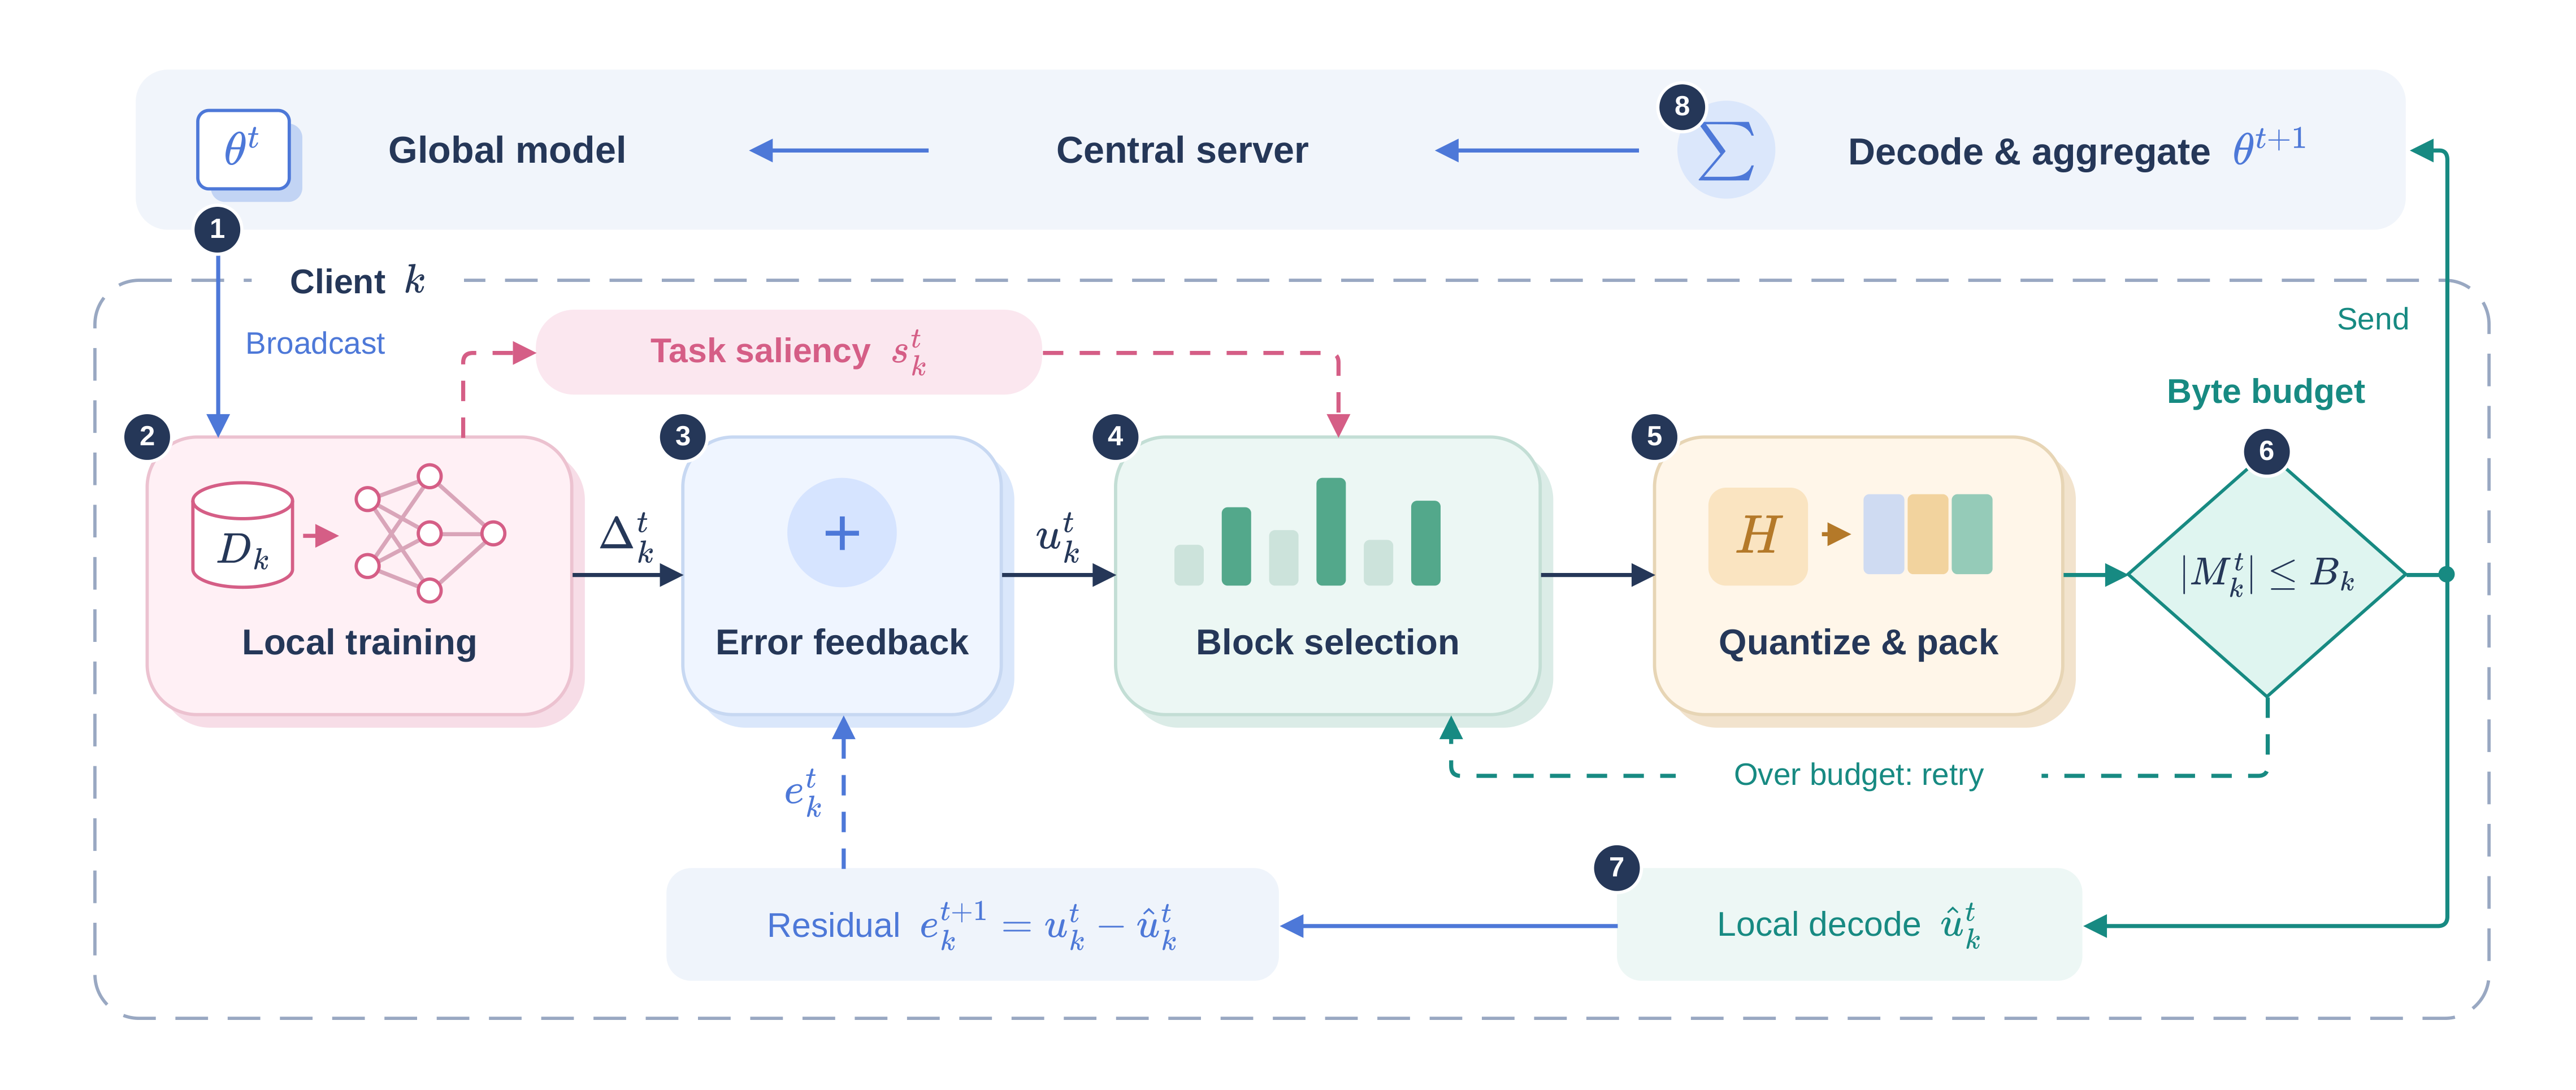
\includegraphics[width=0.85\textwidth]{figures/one_round_fedmpsq_illustrated.png}
  \caption{Round-wise workflow of FedMPSQ}
  \label{fig:method}
\end{figure*}

\subsection{Problem Formulation and FedMPSQ Overview}

\paragraph{Federated IDS setting}
Consider a federated intrusion detection system with $K$ clients, where client
$k$ owns a local training set $D_k$ of size $n_k$ and $n_{k,c}$ samples of
class $c$. At communication round $t$, the server broadcasts the global model
$\theta^t$, each client performs local training, and returns an encoded update
$M_k^t$. Our objective is to retain class-balanced detection utility under a
strict serialized uplink constraint
\begin{equation}
    |M_k^t| \leq B_k,
    \label{eq:budget}
\end{equation}
where $|M_k^t|$ denotes the complete serialized message size in bytes and
$B_k$ is the client uplink budget. The evaluated setting uses full
participation, i.e., all $K$ clients contribute in every round. We assume
cooperative clients and a trusted aggregation server; FedMPSQ does not provide
formal differential-privacy or Byzantine-robustness guarantees.

\paragraph{Class-aware local learning}
To reduce the dominance of frequent attack classes, FedMPSQ adopts
effective-number weighting and logit calibration as the class-aware learning
foundation. Let $N_c=\sum_k n_{k,c}$ denote the pooled training support of
class $c$. For each globally present class,
\begin{equation}
\begin{aligned}
a_c &=
\frac{1-\beta}{1-\beta^{N_c}}, \qquad
\bar a =
\frac{\sum_c N_c a_c}{\sum_c N_c},\\
v_c &=
\operatorname{clip}
\left(
\frac{a_c}{\bar a},
w_{\max}^{-1},
w_{\max}
\right).
\end{aligned}
\label{eq:weights}
\end{equation}
Classes absent from the pooled training set receive zero weight. The
client-specific weight is
\begin{equation}
w_{k,c}
=
\frac{\mathbb{I}[n_{k,c}>0]v_c}{Z_k},
\qquad
Z_k=\frac{1}{n_k}\sum_c n_{k,c}v_c ,
\end{equation}
which normalizes the sample-weighted mean local weight to one.

Let $z_\theta(x)\in\mathbb{R}^{C}$ denote the model logits over the $C$
classes and let $d_k\in\mathbb{R}^{C}$ be the calibration vector with entries
$d_{k,c}=\tau_{\mathrm{LC}}\max(n_{k,c},1)^{-1/4}$, subtracted from all $C$
logits so that the offsets do not cancel inside the softmax. Client $k$
minimizes
\begin{equation}
\mathcal{L}_k^t(\theta)
=
\frac{1}{n_k}
\sum_{(x,y)\in D_k}
w_{k,y}\,
\operatorname{CE}\!\left(z_\theta(x)-d_k,y\right)
+
\frac{\mu}{2}
\|\theta-\theta^t\|_2^2 .
\label{eq:loss}
\end{equation}
The weighting and calibration follow
\cite{cui2019classbalanced,zhang2022fedlc}, while the proximal term follows
FedProx. These components provide the class-aware learning signal used by
FedMPSQ and are not treated as standalone contributions. Calibration is used
only during training; inference uses the unadjusted logits. Pooled class
counts are exchanged once before training, and this one-time metadata cost is
excluded from the reported per-round update traffic.

\paragraph{Round-wise overview}
Fig.~\ref{fig:method} summarizes one communication round of FedMPSQ. The
workflow consists of eight stages. \textbf{(1)} The server broadcasts
$\theta^t$ to all clients. \textbf{(2)} Each client performs class-aware local
training while accumulating a task-sensitivity signal from the gradients of
\eqref{eq:loss}. \textbf{(3)} After local training, the dense model difference
is combined with the residual retained from the previous round.
\textbf{(4)} Task saliency and update magnitude are jointly used to prioritize
coordinates or tensor-local blocks for transmission. \textbf{(5)} The
selected update is quantized and packed into a candidate message.
\textbf{(6)} A controller measures the actual serialized size against the
budget in \eqref{eq:budget}; an over-budget candidate returns to stage~(4)
with a smaller retention level. \textbf{(7)} The accepted message is decoded
locally to form the next residual, and is sent to the server. \textbf{(8)} The
server decodes the received messages and aggregates them into $\theta^{t+1}$.

The design therefore separates two complementary decisions:
\emph{which update information should receive transmission priority} and
\emph{how the retained information should be represented under a strict byte
budget}. The following subsection details these two contribution-bearing
components.

\subsection{FedMPSQ Design Components}

\paragraph{Minority-prioritized task saliency}
During local training, let $g_{k,b}^{\mathrm{task}}$ denote the gradient of the
class-aware data-fitting term in \eqref{eq:loss} for minibatch $b$ containing
$m_b$ samples. For each minibatch, the sensitivity contribution is accumulated
before the SGD update. At the end of the local epoch, these contributions are
averaged and smoothed across communication rounds:
\begin{equation}
\hat{s}_{k,j}^t
=
\frac{
\sum_b m_b
\left|
\theta_{k,j}^{t,b}
g_{k,b,j}^{\mathrm{task}}
\right|
}{
\sum_b m_b
},
\qquad
s_{k,j}^t
=
\eta_s s_{k,j}^{t-1}
+
(1-\eta_s)\hat{s}_{k,j}^t ,
\label{eq:saliency}
\end{equation}
with $s_{k,j}^{0}=0$. The term $|\theta g|$ follows the connection-sensitivity
criterion of SNIP~\cite{lee2019snip}, but FedMPSQ uses it to prioritize
communication rather than prune the model.

Because $g_{k,b}^{\mathrm{task}}$ is induced by the class-aware objective in
\eqref{eq:loss}, underrepresented classes receive greater influence on the
resulting sensitivity signal without requiring an explicit mapping between
classes and model coordinates. The analytical proximal gradient is excluded
from the accumulated saliency so that the score reflects the class-aware task
loss. Importantly, saliency is a task-sensitivity proxy rather than a
guarantee that a particular coordinate belongs to a minority class.

\paragraph{Task-aware sparse update selection}
After local optimization, client $k$ forms
\begin{equation}
\Delta_k^t=\theta_k^t-\theta^t,
\qquad
u_k^t=\Delta_k^t+e_k^t,
\label{eq:residual_input}
\end{equation}
where $e_k^t$ is the reconstruction residual from the previous round. Each
coordinate is then assigned
\begin{equation}
q_{k,j}^t
=
\alpha_s
\frac{s_{k,j}^t}
{\max_i s_{k,i}^t+\epsilon}
+
(1-\alpha_s)
\frac{|u_{k,j}^t|}
{\max_i|u_{k,i}^t|+\epsilon}.
\label{eq:score}
\end{equation}

The two terms encode complementary notions of importance. The saliency term
captures task sensitivity under the class-aware objective, whereas update
magnitude reflects the numerical contribution of the coordinate to the
current local update. Their convex combination prevents transmission decisions
from relying exclusively on either criterion.

FedMPSQ retains the highest-scoring coordinates or tensor-local blocks. For
block selection, scores within each block are aggregated as
$\sum_{j\in\mathcal{B}}(q_{k,j}^t)^2$. Blocks never cross tensor boundaries,
while scalar selection can be used for any remaining byte allowance. Exact
block size and retention settings are reported in the evaluation protocol.

\paragraph{Serialization-aware sparse-quantized encoding}
Let $\mathcal{I}_k^t(r)$ denote the coordinates or blocks retained under a
candidate retention level $r$. The corresponding message is
\begin{equation}
M_k^t(r)
=
\operatorname{Encode}
\left(
u_k^t,\mathcal{I}_k^t(r)
\right),
\qquad
|M_k^t(r)|\leq B_k .
\label{eq:msg}
\end{equation}
Rather than estimating communication from retained parameter counts or
nominal quantization bits, FedMPSQ serializes each candidate and evaluates its
actual byte size, including values, indices, quantization scales, layout
descriptors, headers, and other codec metadata.

Among the feasible candidates considered by the controller, FedMPSQ selects
the one with the smallest reconstruction error,
\begin{equation}
r_k^{t*}
=
\arg\min_{r\in\mathcal{R}_k^t:
|M_k^t(r)|\leq B_k}
\left\|
u_k^t-
\operatorname{Decode}(M_k^t(r))
\right\|_2^2 .
\label{eq:byte_controller}
\end{equation}
Because serialized size need not vary monotonically with the retained count,
the implementation searches a bounded set of candidate retention levels rather
than claiming globally optimal encoding.

The evaluated codec applies a randomized Hadamard transform to retained-value
groups followed by four-level quantization with per-group scales. These codec
settings instantiate the serialization-aware framework; their specific block,
group, and scale parameters are reported in the experimental protocol rather
than treated as methodological contributions.

\paragraph{Error feedback and server aggregation}
Let
\begin{equation}
\hat{u}_k^t
=
\operatorname{Decode}(M_k^t)
\end{equation}
denote the locally reconstructed update. FedMPSQ retains the reconstruction
residual induced by both sparsification and quantization:
\begin{equation}
e_k^{t+1}=u_k^t-\hat{u}_k^t.
\label{eq:feedback}
\end{equation}
The server decodes the received messages and performs sample-weighted
aggregation,
\begin{equation}
\theta^{t+1}
=
\theta^t+
\sum_{k=1}^{K}
\frac{n_k}{\sum_{\ell=1}^{K}n_\ell}
\hat{u}_k^t .
\label{eq:aggregation}
\end{equation}
Error feedback therefore carries information omitted by the current lossy
encoding into subsequent communication rounds
~\cite{karimireddy2019errorfeedback}.

\paragraph{Client-side overhead}
For a model with $P$ parameters, both the saliency state and residual buffer
require $O(P)$ additional client memory. Sparse selection and candidate
serialization also introduce computation, while a Hadamard transform over a
group of width $G$ requires $O(G\log G)$ operations. FedMPSQ therefore targets
\emph{communication efficiency} rather than client-memory reduction, which is
consistent with its positioning as an uplink-efficient federated IDS.

% \section{Proposed Method}
% \subsection{Setting and Local Objective}
% Client $k\in\{1,\ldots,K\}$ has a training set $D_k$ of size $n_k$, with
% $n_{k,c}$ examples of class $c$. A server broadcasts parameters $\theta^t$ at
% round $t$, selects clients $S_t$, and receives encoded local updates
% $M_k^t$. We seek high Macro-F1 and minority recall subject to
% $|M_k^t|\leq B_k$, where $|M_k^t|$ is the number of serialized bytes. We assume
% cooperative clients and a trusted aggregation server; the method provides no
% formal differential-privacy or Byzantine-robustness guarantee.

% The active configurations use pooled training counts $N_c=\sum_k n_{k,c}$
% for effective-number weights. For each globally present class,
% \begin{equation}
%  \begin{aligned}
%  a_c&=\frac{1-\beta}{1-\beta^{N_c}},\qquad
%  \bar a=\frac{\sum_c N_c a_c}{\sum_c N_c},\\
%  v_c&=\operatorname{clip}\!\left(\frac{a_c}{\bar a},w_{\max}^{-1},w_{\max}\right).
%  \end{aligned}
%  \label{eq:weights}
% \end{equation}
% Absent global classes receive zero weight in~\eqref{eq:weights}. Client weights are
% $w_{k,c}=\mathbb{I}[n_{k,c}>0]v_c/Z_k$, where $\mathbb{I}$ is the indicator and
% $Z_k=\sum_c n_{k,c}v_c/n_k$. This normalization keeps the sample-weighted
% mean local weight equal to one. Clipping applies before local normalization,
% so the final weights need not lie in the clipping interval, although their
% nonzero ratio stays bounded by $w_{\max}^2$.

% Let $z_\theta(x)$ be the vector of logits, $\operatorname{CE}$ the
% cross-entropy loss, and $d_k$ the vector with entries
% $d_{k,c}=\tau_{\mathrm{LC}}\max(n_{k,c},1)^{-1/4}$. The local objective is
% \begin{equation}
%  \mathcal L_k^t(\theta)=\frac{1}{n_k}\sum_{(x,y)\in D_k}
%  w_{k,y}\,\operatorname{CE}(z_\theta(x)-d_k,y)
%  +\frac{\mu}{2}\|\theta-\theta^t\|_2^2.
%  \label{eq:loss}
% \end{equation}
% The weighting and calibration follow the ideas
% in~\cite{cui2019classbalanced,zhang2022fedlc}. Calibration is used during
% training; inference uses the model's unadjusted logits. Pooled class counts
% are training-derived metadata; the recorded per-round uplink does not include
% an initial count exchange.

% \subsection{Task Saliency and Sparse Selection}
% Fig.~\ref{fig:method} summarizes the update path. During local training, let
% $g_{k,b}^{\mathrm{task}}$ be the gradient of the first term of
% \eqref{eq:loss} on minibatch $b$, containing $m_b$ examples. Before each SGD
% step we accumulate
% \begin{equation}
%  \hat s_{k,j}^t=\frac{\sum_b m_b
%  |\theta_{k,j}^{t,b}g_{k,b,j}^{\mathrm{task}}|}{\sum_b m_b},\qquad
%  s_{k,j}^t=\eta_s s_{k,j}^{t-1}+(1-\eta_s)\hat s_{k,j}^t.
%  \label{eq:saliency}
% \end{equation}
% The per-coordinate term $|\theta g|$ in~\eqref{eq:saliency} is the connection-sensitivity criterion
% from single-shot pruning~\cite{lee2019snip}; here it is accumulated
% across a round and computed on the class-aware loss, then used to rank
% coordinates for transmission rather than to remove them. The implementation
% subtracts the analytical proximal gradient from the backpropagated objective
% gradient before accumulating saliency. The score is a task-sensitivity proxy,
% not a guarantee that a coordinate belongs to a minority class.

% After training, the local difference is $\Delta_k^t=\theta_k^t-\theta^t$.
% With previous residual $e_k^t$, define $u_k^t=\Delta_k^t+e_k^t$ and
% \begin{equation}
%  q_{k,j}^t=\alpha_s\frac{s_{k,j}^t}{\max_i s_{k,i}^t+\epsilon}
%  +(1-\alpha_s)\frac{|u_{k,j}^t|}{\max_i|u_{k,i}^t|+\epsilon}.
%  \label{eq:score}
% \end{equation}
% Scalar selection retains the largest scores in~\eqref{eq:score}. The block variant partitions each
% flattened tensor into blocks of 32 and ranks them by
% $\sum_{j\in\mathrm{block}}(q_{k,j}^t)^2$; blocks do not cross tensor
% boundaries and a residual allowance uses scalar selection. The nominal
% retained fraction is at most about 10\%, which the byte cap may reduce
% further, so different codecs need not transmit the same number of values.

% \subsection{Byte-Constrained Encoding and Error Feedback}
% \label{sec:encoding}
% The controller serializes candidate retention counts and keeps the feasible
% candidate with the lowest reconstruction error among those tried, using
% boundary checks, a proportional probe, and bounded bisection. Nonmonotonic encoding sizes preclude an optimality guarantee; an
% infeasible minimum payload raises an error.

% The evaluated configuration applies a randomized Hadamard transform (RHT) to
% full groups of 256 retained values with a four-centroid codebook, about
% $\{-1.5104,-0.4528,0.4528,1.5104\}$ (denoted G4, i.e.\ two-bit values).
% Per-group scales are fitted by reconstruction error and encoded
% logarithmically in one byte, code assignments use the decoded scales, short
% trailing groups are left unrotated, and decoder-reproducible signs depend on
% client, round, and tensor identifiers.

% Writing $\hat u_k^t=\operatorname{Decode}(M_k^t)$, the residual and server
% update are
% \begin{equation}
%  e_k^{t+1}=u_k^t-\hat u_k^t,\qquad
%  \theta^{t+1}=\theta^t+
%  \sum_{k\in S_t}\frac{n_k}{\sum_{\ell\in S_t}n_\ell}\hat u_k^t.
%  \label{eq:feedback}
% \end{equation}
% Equation~\eqref{eq:feedback} corrects both dropped coordinates and
% quantization error~\cite{karimireddy2019errorfeedback}. Serialized bytes
% include values, indices, scales, layout descriptors, headers, and metadata. Saliency and
% residual storage each require $O(P)$ memory for $P$ parameters. Selection and
% repeated encoding add computation; a Hadamard group of width $G$ costs
% $O(G\log G)$.

\section{Implementation and Experiments}
\subsection{Evaluation Protocol}
\paragraph{Experiment Settings}
All experiments are conducted on Kaggle Notebooks using PyTorch 2.10.0,
CUDA 12.8, and NVIDIA Tesla T4 GPUs, with seed 42 for reproducibility.
The same environment is used across all configurations.

\paragraph{Data and partitions}
We use all 46 features and 34 labels of CICIoT2023~\cite{neto2023ciciot2023}.
The dataset is first randomly split into 80\% training data and a fixed 20\%
global test set. The training portion is then independently partitioned into
$K=10$ and $K=100$ clients using Python's Mersenne Twister pseudo-random
generator with a fixed seed of 42 to ensure reproducibility. The resulting
client partitions exhibit heterogeneous class distributions and unequal local
class support, as illustrated in Fig.~\ref{fig:label_distribution}. The global
test set remains fixed and is shared by all methods.
\begin{figure*}[ht]
    \centering
    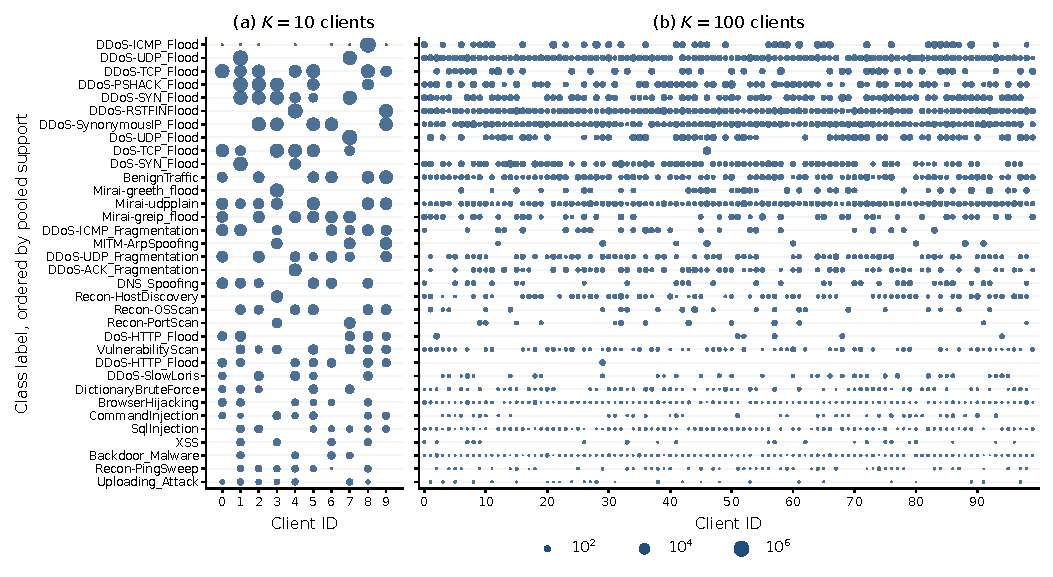
\includegraphics[width=0.8\textwidth]{figures/label_bubbles.pdf}
    \caption{Client-level label distributions for $K=10$ and $K=100$. Class labels are ordered by pooled training support, and bubble size represents the number of samples assigned to each client--class pair.}
    \label{fig:label_distribution}
\end{figure*}

\paragraph{Metrics and evaluation}
We report Accuracy (Acc), Macro-Recall (M-R) Macro-$F_1$-Score (M-$F_1$), Weighted-Recall (W-R) and Weighted-$F_1$-Score (W-$F_1$), emphasizing M-$F_1$ under class imbalance.

\paragraph{Common training setup}
All methods use the same DCNN--BiLSTM classifier with convolutional channels
64/128/128, kernel size 3, a bidirectional LSTM with hidden size 128,
LayerNorm, and dropout 0.2. The FP32 model contains 348,322 parameters and
occupies 1,393,288 bytes. Training uses full client participation, one local
epoch per round, batch size 256, and SGD with learning rate $10^{-3}$,
momentum 0.9, and weight decay $10^{-4}$. FedProx-based methods use
$\mu=0.01$. 

\paragraph{Baselines}
FedAvg and FedProx are used as dense references
~\cite{mcmahan2017fedavg,li2020fedprox}. We further compare against
BDD-HFL~\cite{song2024bddhfl}, FAP~\cite{wang2025fapdp},
FedPAQ~\cite{reisizadeh2020fedpaq}, and
DAdaQuant~\cite{honig2022dadaquant} under the same training budget.
BDD-HFL and FAP are evaluated with both aggregation backbones: the unmarked
variants use FedAvg, whereas the superscript $\mu$ denotes their FedProx-based
counterparts with proximal coefficient $\mu=0.01$. FedPAQ follows the FedAvg
backbone, while DAdaQuant and FedMPSQ use FedProx.

\paragraph{FedMPSQ configuration}
FedMPSQ uses the FedProx backbone with $\mu=0.01$,
$\beta=0.9999$, $w_{\max}=10$, $\tau_{\mathrm{LC}}=1$,
$\eta_s=0.9$, and $\alpha_s=0.25$, together with pooled training priors and
error feedback. The evaluated RHT-G4 codec uses blocks of 32, transform groups
of 256 values, and one-byte logarithmic scales. All hyperparameters are fixed
across federation scales; only the serialized uplink budget changes from
3,334 bytes per client per round for $K=10$ to 3,044 bytes for $K=100$.

\subsection{Results}

\begin{table}[ht]
\centering
\footnotesize
\caption{Global detection performance at round 20.}
\label{tab:main}

\begin{tabular}{clrrrrr}
\toprule
$K$ & Method & Acc & M-R & W-$R$ & M-$F_1$ & W-$F_1$ \\
\midrule
\multirow{9}{*}{10} & FedAvg & 74.53 & 45.12 & 74.53 & 38.36 & 67.13 \\
 & FedProx & 75.56 & 44.41 & 75.56 & 36.98 & 68.06 \\
 & BDD-HFL & 61.92 & 40.38 & 61.92 & 31.83 & 53.33 \\
 & BDD-HFL$^{\mu}$ & 73.03 & 42.78 & 73.03 & 35.41 & 65.32 \\
 & FAP & 75.44 & 44.16 & 75.44 & 37.24 & 67.68 \\
 & FAP$^{\mu}$ & 75.47 & 44.92 & 75.47 & 37.90 & 67.89 \\
 & FedPAQ & 71.50 & 42.14 & 71.50 & 35.70 & 64.84 \\
 & DAdaQuant & \textbf{75.94} & 45.01 & \textbf{75.94} & 38.05 & \textbf{69.48} \\
 & \textbf{\method{}} & 75.12 & \textbf{47.41} & 75.12 & \textbf{39.17} & 67.71 \\
\midrule
\multirow{9}{*}{100} & FedAvg & 74.91 & 40.49 & 74.91 & 37.85 & 69.42 \\
 & FedProx & 74.87 & 40.46 & 74.87 & 37.96 & 69.45 \\
 & BDD-HFL & 71.01 & 32.88 & 71.01 & 27.52 & 62.93 \\
 & BDD-HFL$^{\mu}$ & 71.12 & 32.91 & 71.12 & 27.57 & 63.09 \\
 & FAP & 74.82 & 40.16 & 74.82 & 37.77 & 69.34 \\
 & FAP$^{\mu}$ & 74.72 & 40.15 & 74.72 & 37.86 & 69.31 \\
 & FedPAQ & 74.89 & 40.40 & 74.89 & 37.43 & 69.21 \\
 & DAdaQuant & 74.82 & 40.28 & 74.82 & 37.49 & 69.15 \\
 & \textbf{\method{}} & \textbf{78.56} & \textbf{41.44} & \textbf{78.56} & \textbf{38.91} & \textbf{72.96} \\

\bottomrule
\end{tabular}
\end{table}

\paragraph{Detection performance}
Table~\ref{tab:main} reports the final performance after 20 communication
rounds. For $K=10$, FedMPSQ achieves the highest M-$F_1$ (39.17\%) and
M-R (47.41\%), exceeding the strongest baselines by 0.81 and 2.29
percentage points, respectively. Its Accuracy remains competitive at 75.12\%,
while DAdaQuant attains the highest Accuracy (75.94\%) and W-$F_1$
(69.48\%). Under the evaluated class-imbalanced setting, FedMPSQ therefore provides
stronger class-balanced utility while retaining competitive aggregate
performance.

For $K=100$, FedMPSQ achieves the highest final values across all reported
metrics, reaching 78.56\% Accuracy, 41.44\% M-R, 38.91\%
M-$F_1$, and 72.96\% W-$F_1$. Compared with the strongest baseline
for each metric, the corresponding gains are 3.65, 0.95, 0.95, and 3.51
percentage points. Most competing methods remain close to 75\% Accuracy,
approximately 40\% M-R, and below 38\% M-$F_1$. These results
show that the substantially smaller uplink of FedMPSQ is observed without a
corresponding reduction in final detection utility and, at $K=100$, coincides
with higher final values across all reported metrics.

\begin{figure*}[ht]
\centering
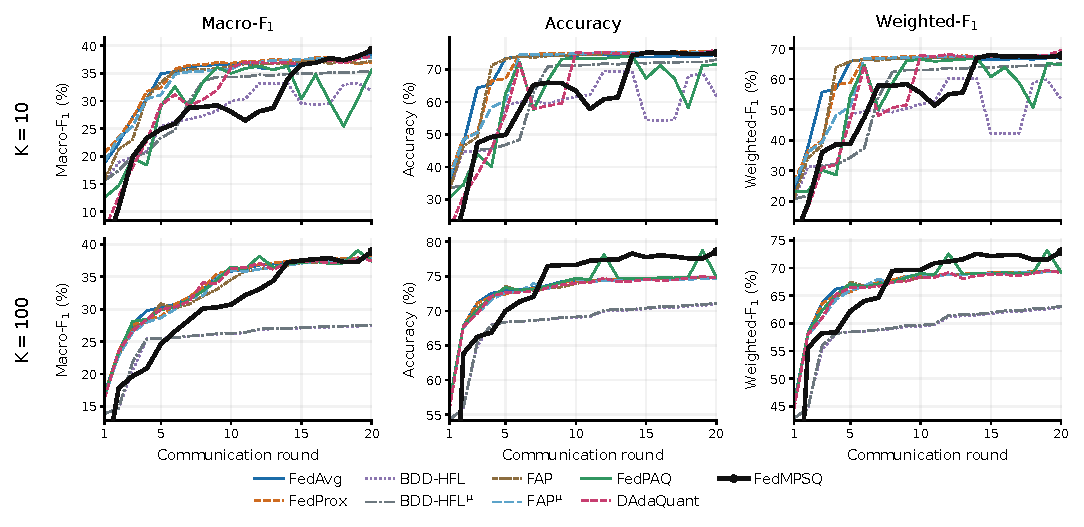
\includegraphics[width=0.9\textwidth]{figures/metrics_rounds.pdf}
\caption{Round-wise detection performance of all methods under the two federation scales, $K=10$ and $K=100$.}
\label{fig:f1rounds}
\end{figure*}

\paragraph{Class-balanced and round-wise behavior}
The higher M-R and M-$F_1$ indicate that FedMPSQ maintains
utility across classes while keeping its frequency-weighted metrics
competitive. These results should be interpreted as improved class-balanced
behavior rather than guaranteed preservation of every rare class.

Fig.~\ref{fig:f1rounds} further shows that FedMPSQ improves more gradually in
the early rounds, with its M-$F_1$ gap narrowing as training proceeds.
At $K=10$, its M-$F_1$ rises in the later rounds and finishes with the
highest final value, while at $K=100$ it finishes with the highest values
across all three plotted metrics. This late-round improvement is compatible
with the iterative sparse-update and residual-correction design of FedMPSQ,
although dedicated ablations are needed to isolate the effects of individual
components.

\begin{table}[ht]
\centering
\footnotesize
\caption{Average communication cost per client per round across the two
federation scales, in decimal KB ($10^{3}$~B).}
\label{tab:comm}

\resizebox{\columnwidth}{!}{%
\begin{tabular}{lccrrr}
\toprule
\textbf{Method}
& \textbf{\makecell{Upload\\payload}}
& \textbf{\makecell{Download\\payload}}
& \textbf{\makecell{Upload\\(KB)}}
& \textbf{\makecell{Download\\(KB)}}
& \textbf{$\Delta_{Upload}$} \\
\midrule

FedAvg
& $|\theta_i|$
& $|\theta_g|$
& 1397.020
& 1397.020
& $438.8\times$ \\

FedProx
& $|\theta_i|$
& $|\theta_g|$
& 1397.020
& 1397.020
& $438.8\times$ \\

BDD-HFL
& $|\theta_i|$
& $|\theta_g|$
& 1397.020
& 1397.020
& $438.8\times$ \\

BDD-HFL$^{\mu}$
& $|\theta_i|$
& $|\theta_g|$
& 1397.020
& 1397.020
& $438.8\times$ \\

FAP
& $|\theta_i|$
& $|\theta_g|$
& 1397.020
& 1397.020
& $438.8\times$ \\

FAP$^{\mu}$
& $|\theta_i|$
& $|\theta_g|$
& 1397.020
& 1397.020
& $438.8\times$ \\

FedPAQ
& $|Q(\Delta\theta_i)|$
& $|\theta_g|$
& 176.508
& 1397.020
& $55.4\times$ \\

DAdaQuant
& $|Q_{b_i^t}(\Delta\theta_i)|$
& $|\theta_g|$
& 4.924
& 1397.020
& $1.55\times$ \\

\textbf{FedMPSQ}
& $|M_i^t|$
& $|\theta_g|$
& \textbf{3.184}
& 1397.020
& \textbf{$1.00\times$} \\

\bottomrule
\end{tabular}%
}
\end{table}

\paragraph{Communication efficiency}
The largest quantitative margin of FedMPSQ appears in serialized client
uplink. For compact reporting, Table~\ref{tab:comm} averages the per-client,
per-round communication cost equally across the two federation scenarios.
FedMPSQ transmits only 3.184~KB per client per round, compared with 4.924~KB
for DAdaQuant, 176.508~KB for FedPAQ, and 1397.020~KB for dense model
transmission. This corresponds to uplink reductions of approximately 35.3\%,
98.2\%, and 99.77\%, respectively; equivalently, these alternatives require approximately
1.55$\times$, 55.4$\times$, and 438.8$\times$ as much uplink as FedMPSQ.

DAdaQuant provides the closest comparison in terms of serialized uplink cost.
FedMPSQ uses 35.3\% less uplink while achieving a 1.12 percentage-point higher
M-$F_1$ and a 2.40-point higher M-R at $K=10$. At $K=100$, it
achieves higher Accuracy, M-R, M-$F_1$, and W-$F_1$.
Hence, the communication saving is not obtained merely by sacrificing
predictive utility; on the reported average-uplink basis, FedMPSQ provides a
more favorable observed utility--uplink trade-off than DAdaQuant under the
evaluated settings.

The reduction specifically concerns \emph{client-to-server communication}.
All methods still download the same dense FP32 global model
(1397.020~KB per client per round). FedMPSQ should therefore be interpreted as
an uplink-efficient federated IDS rather than a fully bidirectional lightweight
communication scheme.

\paragraph{Overall findings and practical implications}
Overall, FedMPSQ retains competitive detection utility under a highly
constrained serialized uplink budget while improving class-balanced
performance. Its low communication footprint is particularly relevant to
bandwidth-constrained federated IDS deployments, where repeated client uploads
can become a major bottleneck. However, the current evaluation targets uplink
only; dense downlink, latency, memory, energy consumption, and device-level
execution remain outside the present scope. These limitations motivate
bidirectional compression, adaptive byte budgets, and resource-aware client
participation as natural extensions.

\section{Conclusion}
This work introduced FedMPSQ, an uplink-efficient federated IDS that formulates
compression as a task-aware resource-allocation problem. By combining
class-aware update prioritization, serialization-aware sparse quantization, and
residual correction, FedMPSQ achieves a favorable utility--uplink trade-off
under non-IID settings.
FedMPSQ attains the highest M-$F_1$ and M-R at $K=10$ and the
highest observed final values across all reported metrics at $K=100$, while
requiring only 3.184~KB of mean serialized uplink per client per round. This
corresponds to reductions of 35.3\% relative to DAdaQuant and 99.77\% relative
to dense FL.
FedMPSQ should nevertheless be interpreted as uplink-efficient rather than
fully lightweight, since the downlink remains dense and class-balanced gains do
not guarantee preservation of every rare class. Future work will investigate
bidirectional compression, adaptive byte budgets, resource-aware participation,
and multi-seed and component-level evaluations.

\section*{Acknowledgements} 
This research was supported by The VNUHCM-University of Information Technology's Scientific Research Support Fund.

\bibliographystyle{IEEEtran}
\bibliography{\paperassets/references}
\end{document}

